\documentclass[12pt,fullpage]{amsart}
\usepackage{enumerate,graphicx,fullpage, multicol}
\graphicspath{{../images/}}
\input{/home/treisman/tex/macros}


\pagestyle{empty}
\setlength{\parindent}{0pt}
\newcommand{\ds}{\displaystyle}
\begin{document}

\begin{center}\textbf{Statistics Review Questions \quad\ddag\quad Spring 2021}
\end{center}

\hrulefill
\medskip
\begin{enumerate}

\item You have been tasked with collecting data on the herd of bighorn sheep that live in the Almont Triangle.
\begin{enumerate}
  
\item Describe a data set that you will collect.
  \begin{enumerate}
  \item What are the cases or observations?
  \item What are three possible variables? 
  \end{enumerate}
    
\item For each of your three variables: is it categorical or numerical?

\item Give a question that you could ask about a possible correlation between two variables in these data. 

\item For your question directly above, what are the explanatory and response variables?

\end{enumerate}
  
\item The values 110 110  93 110 175 105 245  62  95 123 123 180 180 180 205 215 230  66  52  65  97 150 150 245 175  66  91 113 264 175 335 109 are the horsepower ratings of 32 cars, (Data are from \texttt{mtcars\$hp} in the data included with the R software.)
Find the 
\begin{multicols}{3}
\begin{enumerate}
\item mean

\item median

\item standard deviation

\item Q1

\item Q3

\end{enumerate}
\end{multicols}


\item For the variable whose histogram is shown below, which statistic should you use to report the center of the distribution?  Which statistic should you use to report the spread? Why?

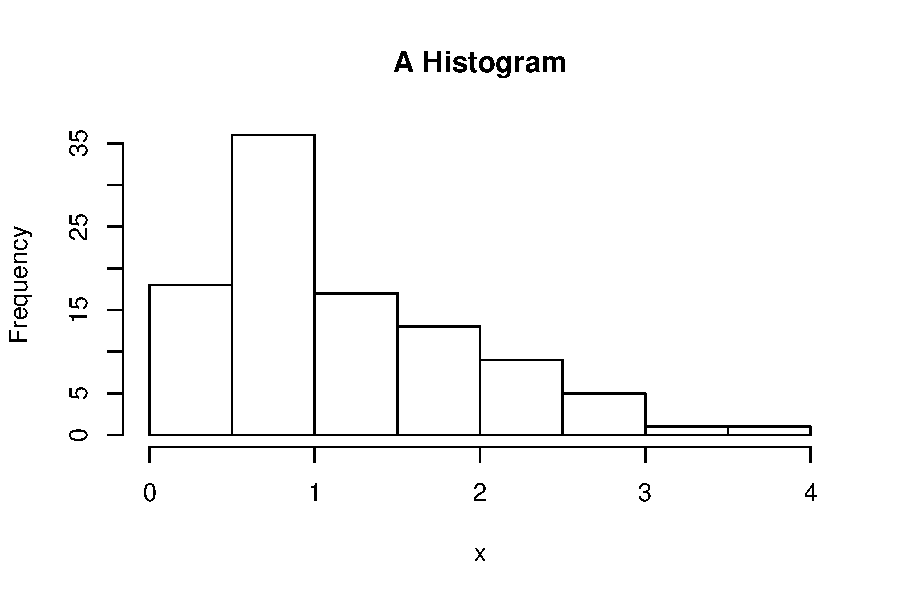
\includegraphics[scale=0.5]{RightSkew}


\item The length of the thorax of a population of fruit flies is
  normally distributed with mean 0.8 mm and standard deviation 0.078
  mm.
  \begin{enumerate}
  \item What proportion of the fruit flies have thorax length less
    than 0.72 mm?
  \item What proportion of the fruit flies have thorax length greater
    than 0.82 mm?
  \item What proportion of the fruit flies have thorax length between
    0.7 and 0.9 mm?
  \item We wish to select the fruit flies with the highest 20\% of
    thorax length.  What is the shortest thorax length we should
    consider?
  \end{enumerate}

 \newpage
 

\item
This table represents the first 3 observations from a sample of 2000 results from the US Census American Community Survey, 2012. Individuals reported their annual income, age, gender, marital status and education level.
\begin{table}[ht]
\centering
\begin{tabular}{rrrlll}
  \hline
 & income & age & gender & married & edu \\ 
  \hline
1 & 60000 &  68 & female & no & college \\ 
  2 &   0 &  88 & male & no & hs or lower \\ 
  3 &  0 &  12 & female & no & hs or lower \\ 
   \hline
\end{tabular}
\end{table}
\begin{enumerate}
\item Which of these five variables are numerical? (There may be none or more than one.)
  \begin{multicols}{3}
  \begin{enumerate}
  \item \texttt{income}
  \item \texttt{age}
  \item  \texttt{gender}
  \item \texttt{married}
  \item \texttt{edu}
  \end{enumerate}
  \end{multicols}
\item Which type of plot would be appopriate to use to view the relationship between \texttt{income} and \texttt{gender}? (There may be none or more than one.)
  \begin{multicols}{3}
\begin{enumerate}
\item single histogram
\item hollow histograms
\item single boxplot
\item side by side boxplot
\item scatter plot
\end{enumerate}
  \end{multicols}
\item
Below are some summary statistics from the \texttt{age} variable.
\begin{verbatim}
 Min.   1st Qu. Median  Mean    3rd Qu.    Max.         St. Dev.
 0.00   19.75   40.00   40.22   59.00      94.00        23.66
\end{verbatim}
Which of the following is \underline{true}? (There may be none or more than one.)
\begin{enumerate}
    \item
      The standard deviation and the inter quartile range give similar information.
    \item
    There is little or no evidence that the distribution of \texttt{age} is skewed.
    \item
    The minimum value of 0 would be identified as out outlier in a box plot.
    \item
    Half of the individuals are between 19.75 and 59 years old.
      
\end{enumerate}


\item Here is a side by side boxplot of the \texttt{edu} and \texttt{income} variables.

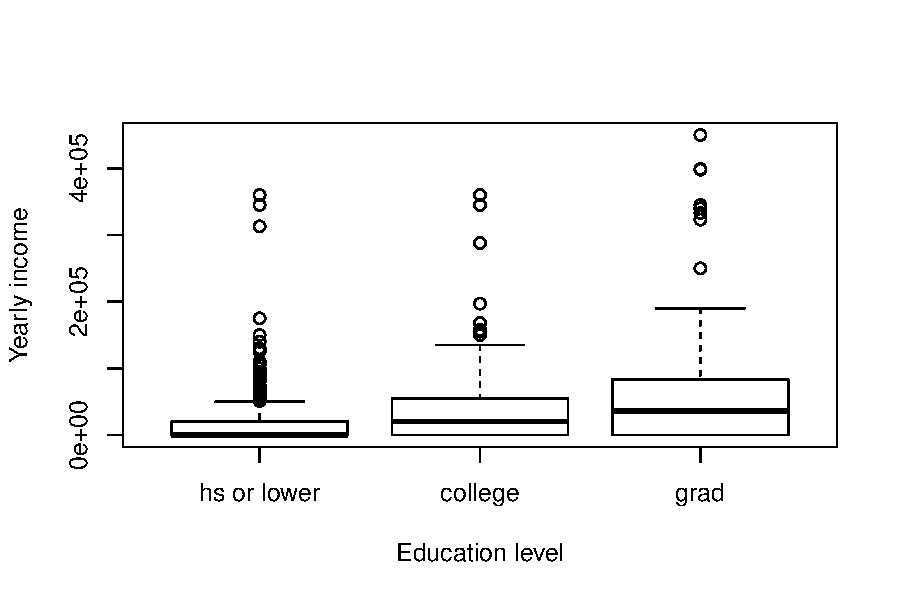
\includegraphics[scale=0.45]{eduIncome}

Which of the following is \underline{true}? (There may be none or more than one.)

\begin{enumerate}
\item The data show no difference in yearly income between different education levels.
\item There are more outliers in \texttt{income} for \texttt{grad} than for \texttt{hs or lower}.
\item The data are right-skewed in all three groups.
\item The inter quartile range is greater for \texttt{hs or lower} than for \texttt{grad}.
\end{enumerate}

\end{enumerate}


\item In the 2010 election, John Hickenlooper won 51 percent of the votes in Colorado. A pollster takes a survey of Colorado voters who voted in the 2010 election and finds that 48 percent of those surveyed voted for Hicknlooper in 2010.

  \begin{enumerate}
  \item The 51 percent is a \blank[2cm] and the 48 percent is a \blank[2cm].
\begin{multicols}{3}
    \begin{enumerate}
\item   statistic; parameter
\item	parameter; statistic
\item	population; sample
\item sample; population
\item none of the above
    \end{enumerate}
\end{multicols}

\item The people who voted in the 2010 election is the \blank[2cm] and the people the pollster talked to is a \blank[2cm].
  \begin{multicols}{3}
    \begin{enumerate}
\item   statistic; parameter
\item	parameter; statistic
\item	population; sample
\item sample; population
\item none of the above
\end{enumerate}
  \end{multicols}
  \end{enumerate}

  
\item
Based on a random sample of 120 rhesus monkeys, a 95\% confidence interval for the proportion of rhesus monkeys that live in a captive breeding facility and were assigned to research studies is (0.67, 0.83).  Which of the following is \underline{true}?
\begin{enumerate}
\item	95 of the sampled monkeys were assigned to research studies
\item	the margin of error for the confidence interval is 0.16
\item	a larger sample size would yield a wider confidence interval
\item	if we used a different confidence level, the interval would not be symmetric about the sample proportion
\item	none of the above are true
\end{enumerate}

  
\item
  Approximately 19\% of physics majors in the US are women. Western doesn't have a physics major, but we might start one. To test whether we differ significantly from this national average, you take a random sample of 50 Western students who say they would consider a physics major and find that 23 are female.
  \begin{enumerate}
  \item What is your point estimate for the proportion of Western students who would consider a physics major who are female?
  \item Using a normal model for the proportion, what is the standard error in your estimate?
    \item Give a 95\% confidence interval for the proportion of potential physics majors at Western who are female.
    \item If you would like your margin of error to be at most $\pm 5\%$, assuming that the proportion of potential physics majors who are female does not change, how many potential physics majors would you have to include in your sample?
  \end{enumerate}
  
\item
Complete the following sentence: When conducting a hypothesis test, we \underline{\hspace{1in}} and then evaluate the test results to determine if there is enough evidence to \underline{\hspace{1in}}.
\begin{enumerate}
\item	Assume that the null hypothesis is false; accept the null hypothesis
\item	Assume that the null hypothesis is true; reject the null hypothesis
\item	Assume that the alternative hypothesis is true; reject the null hypothesis
\item	Assume the alternative hypothesis is false; reject the alternative hypothesis
\end{enumerate}

\item A coin is flipped 1000 times. It comes up heads 532 times. Is this a fair coin?
  \begin{enumerate}
  \item Give appropriate null and alternative hypotheses.
  \item Give the test statistic, degrees of freedom if appropriate, and $p$-value for the test.
\item Give a 95\% confidence interval for the probability that the coin comes up heads.
  \item Clearly interpret your results in a sentence.
  \end{enumerate}

\item An ecologist hypothesizes that a lake's fish population is stable when the ratios of three types of fish are 10:5:2. The ecologist samples the fish in the lake collects the following data.

%\begin{center}
\begin{tabular}{ll}
\textbf{fish type} & \textbf{count}\\
\hline
fish A & 650\\
fish B & 412\\
fish C & 120\\
\hline
\textbf{total} & 1182
\end{tabular}
%\end{center}

Do a hypothesis test using the $\chi^2$ statistic to evaluate this model.
\begin{enumerate}
  \item What are your null and alternate hypotheses?
  \item How many of fish A do we expect to find out of 1182 total fish if the 10:5:2 model is correct?
  \item What are the degrees of freedom, the $\chi^2$ statistic, and the $p$-value?
\item What is your conclusion based on your test?
  \end{enumerate}

\item An ecologist wants to know if the distributions of three types of fish are the same in two lakes. She collects the following data.

%\begin{center}
\begin{tabular}{llll}
\textbf{fish type} & \textbf{Blue Lake} & \textbf{Green Lake} & \textbf{totals}\\
\hline
fish A & 650 & 408 & 1058\\
fish B & 412 & 387 & 799\\
fish C & 120 & 68 & 188\\
\hline
\textbf{totals} & 1182 & 863 & 2045
\end{tabular}
%\end{center}

Do a hypothesis test using the $\chi^2$ statistic.
\begin{enumerate}
  \item What are your null and alternate hypotheses?
  \item How many of fish A do we expect to see in Green Lake if the distributions are the same in both lakes?
  \item What are the degrees of freedom, the $\chi^2$ statistic, and the $p$-value?
\item Do you think that the distributions of fish types are the same in both lakes? Explain.
\end{enumerate}


\item Researchers measured the metabolic rate (in kCal/day) for 12 participants in a study.  The measurements recorded were as follows: 995 1425 1396 1418 1502 1256 1189  913 1124 1052 1347 1204.

  The researchers would like to know if the metabolic rates for this group differ from the presumed baseline metabolic rate of 1500 kCal/day.


  \begin{enumerate}
  \item Give appropriate null and alternative hypotheses.
  \item Give the test statistic, degrees of freedom, and $p$-value for
    the test.
\item Give a 95\% confidence interval for the mean metabolic rate in this group.
  \item Clearly interpret your results in a sentence.
  \end{enumerate}




\item Road tests of 32 cars produced data, included in R as the \texttt{mtcars} dataset, including horsepower and gas mileage. The output of a linear model is shown.

%\begin{center}
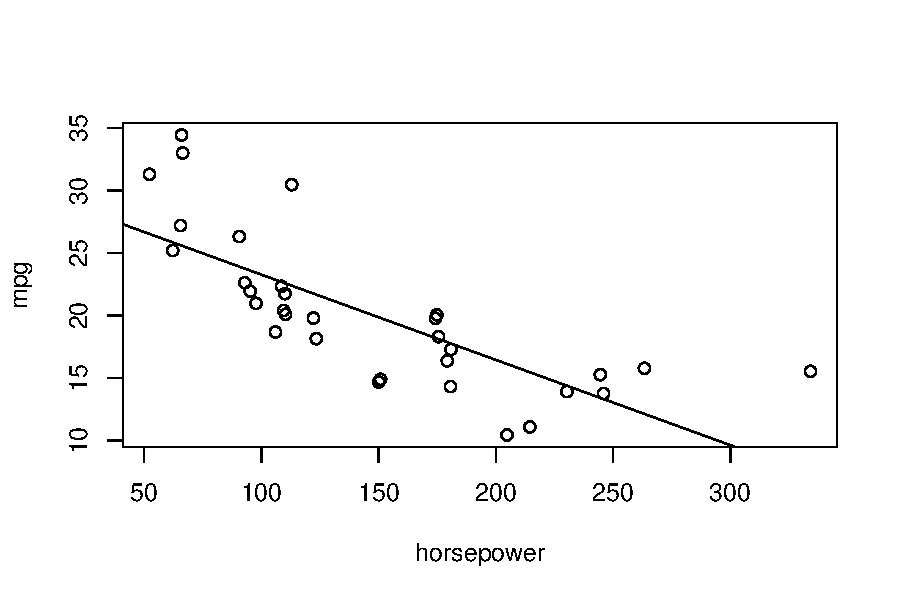
\includegraphics[width=10cm]{cars}
%\end{center}

\begin{verbatim}
Coefficients:
            Estimate Std. Error t value Pr(>|t|)    
(Intercept) 30.09886    1.63392  18.421  < 2e-16 ***
mtcars$hp     -0.06823    0.01012  -6.742 1.79e-07 ***
\end{verbatim}

  \begin{enumerate}
  \item What was the null hypotheses tested for the \texttt{mtcars\$hp} coefficient?

  \item What can you conclude about the relationship between horsepower and gas mileage?

\item One of the assumptions that underlies linear regression is that the residuals are normally distributed and do not depend on the explanatory variable. Is this assumption satisfied by this model? Explain.

  \end{enumerate}


\item Data are in \texttt{mtcars}. The same data set also contains the number of cylinders for each car and the time in seconds for each car to travel a quarter mile, starting from a stop, in seconds.  Summary statistics for the quarter mile time for the 4, 6, and 8 cylinder cars are:
\bigskip


\begin{tabular}{c|ccccccc}
cylinders & Min. & 1st Qu. & Median & Mean & 3rd Qu. & Max. & sd\\
\hline
4 & 16.70 & 18.56 & 18.90 & 19.14 & 19.95 & 22.90 & 1.68\\
6 & 15.50 & 16.74 & 18.30 & 17.98 & 19.17 & 20.22 & 1.71\\
8 & 14.50 & 16.10 & 17.18 & 16.77 & 17.55 & 18.00 & 1.20
\end{tabular}

  \begin{enumerate}
  \item Make a plot comparing the quarter mile times for the different size engines. Does it look like there is a difference?
  \item Are the conditions for ANOVA satisfied? Explain.

  \item Here is the output of doing ANOVA. Based on this test, what can you conclude about the
    relationship between number of cylinders and quarter mile times? 
    \begin{verbatim}
                  Df Sum Sq Mean Sq F value  Pr(>F)   
factor(mtcars$cyl)  2  34.61   17.30   7.794 0.00196 **
Residuals          29  64.38    2.22
\end{verbatim}

  \end{enumerate}


\item Veterinarians at a nonhuman primate research center are interested in estimating the true average birth weight of rhesus monkeys born in captivity.  Below are the summary statistics of the data and output from the analysis testing if the true average birth weight of the monkeys is 0.4kg.  What is the correct calculation to estimate the true average birth weight of rhesus monkeys with a 95\% confidence interval?
\begin{verbatim}
  min   Q1 median  Q3  max mean   sd  n missing
 0.27 0.37   0.39 0.5 0.68 0.44 0.12 10       0

t = 1.0853, df = 9, p-value = 0.306
alternative hypothesis: true mean is not equal to 0.4
95 percent confidence interval:
 XXXXXXX XXXXXXX
\end{verbatim}
\begin{enumerate}
\item	$0.44 \pm 1.0853 \times 0.12 / \sqrt{9} $
\item	$0.44 \pm 1.0853 \times 0.12  $
\item	$0.44 \pm 2.26 \times 0.12 / \sqrt{10} $
\item	$0.39 \pm 1.96 \times 0.12 $
\item  $0.39 \pm 2.26 \times 0.12 / \sqrt{9} $
\end{enumerate}

\item An ecologist researching Monarch butterfly migration studies the relationship between wing weight in milligrams and wing area in square millimeters. A scatterplot of the data along with a linear regression line are shown below.  This line has equation $y = 395.01 + 38.23 x$ and correlation coefficient $r=0.802$
  \begin{enumerate}
  \item Do you trust the regression line?  Why or why not?

  \item What is the biological meaning of the intercept 395.01?  Do
    you trust this?  Why or why not?

  \item What is the biological meaning of the slope 38.23?

  \item What does the model predict for the area of a wing weighing 10 milligrams?

  \end{enumerate}
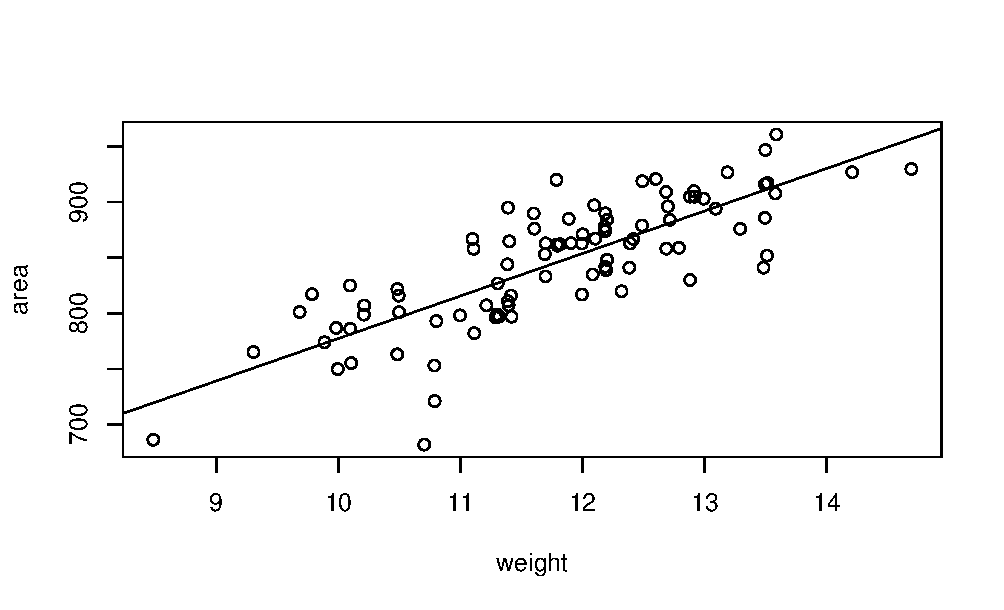
\includegraphics[scale=0.7]{areaWeight}



\end{enumerate}
\end{document}
